\chapter{Application outline}
\label{ch:outline}

Throughout this project, an implementation of the application has been planned. This chapter outlines how such an implementation may look like.

\section{Implementation details}

Following the reasoning in \autoref{sec:iteration6} and \autoref{sec:appsetup}, the current approach is to split the application in two; an web application for patients (optimized for tablets) and a web application for the staff (optimized for desktop). The avatar generation system is to be integrated into both applications. An extended use case diagram is shown in \autoref{fig:usecases2} to reflect these changes.

\begin{figure}
    \centering
    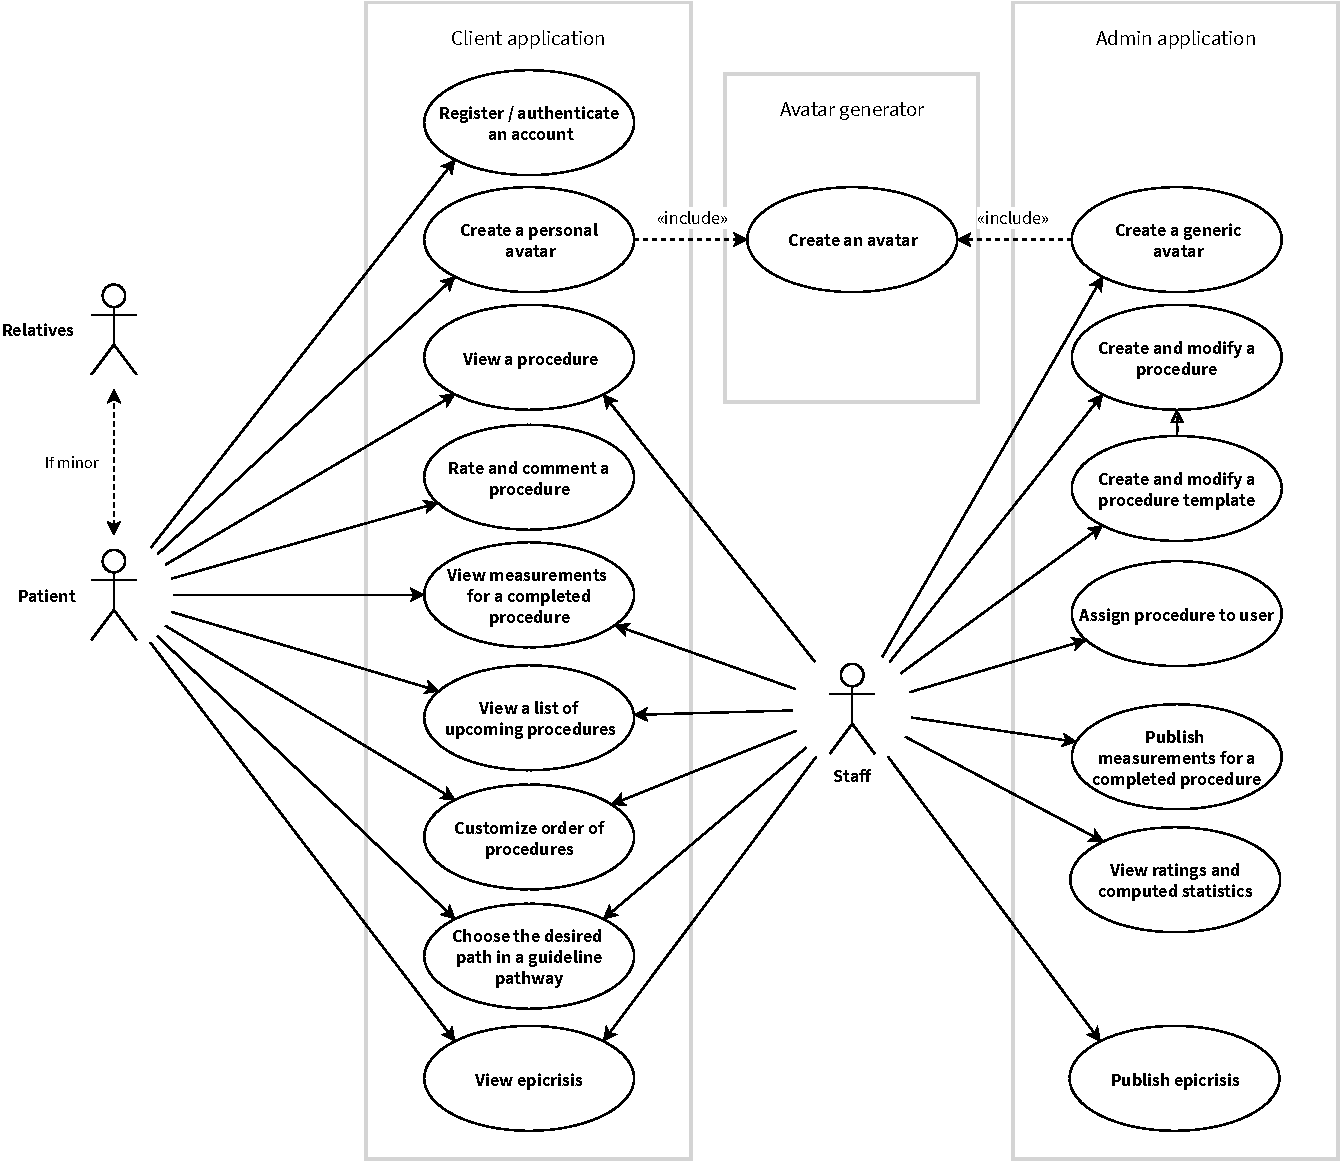
\includegraphics[width=1\textwidth]{use-cases-implementation.pdf}
    \caption{Extended use case diagram}
    \label{fig:usecases2}
\end{figure}

A revised and more detailed domain model is shown in \autoref{fig:domainmodel2}. Here, the concepts of the domain are further analysed and made more concrete. A procedure is now made up of several \emph{pages} and a textual \emph{document}. Each page may include a drawing, a video or an image depending on its source. The user's avatar is only displayed in a DrawingPage. The concepts of PictogramApp (stories and scenes) are carried over to the application as well, although named as \emph{procedures} and \emph{steps} respectively.

\begin{figure}
    \centering
    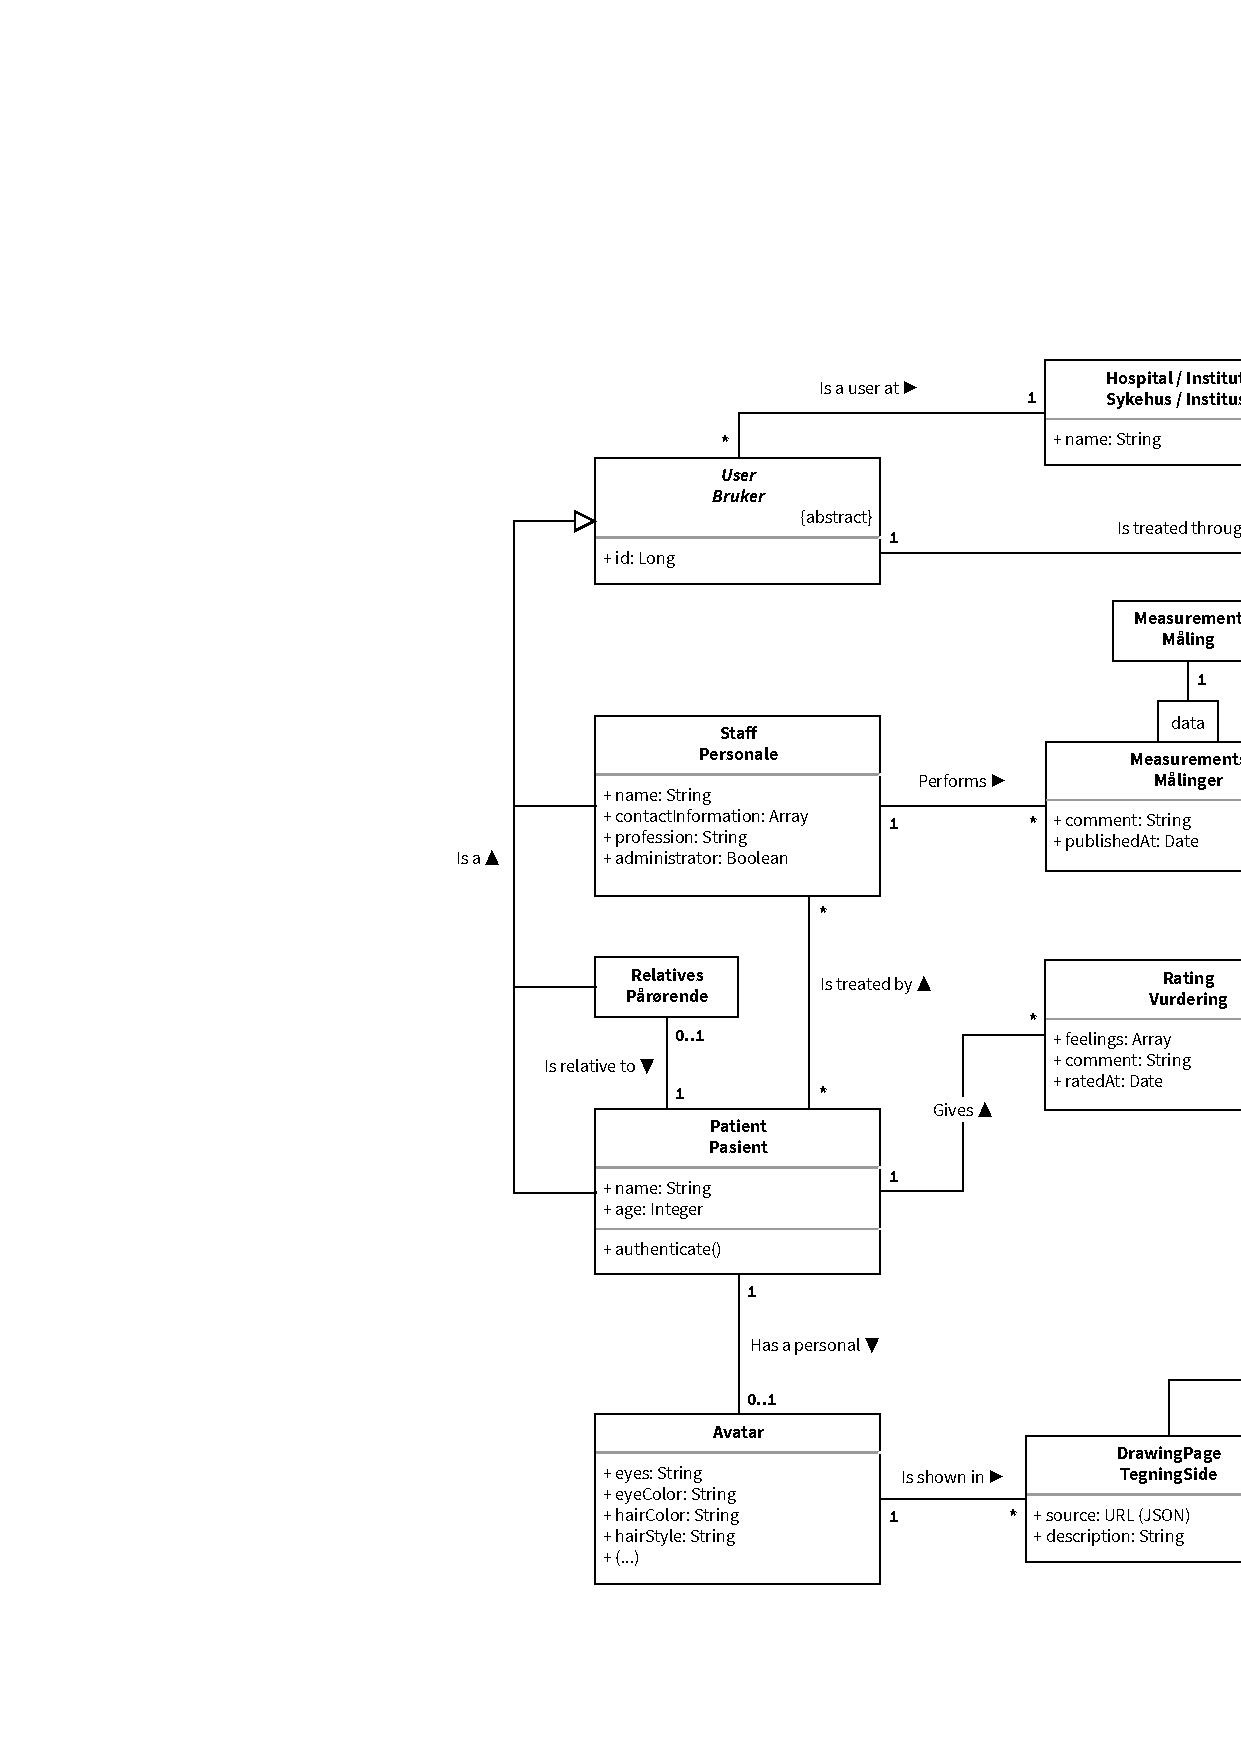
\includegraphics[width=1\textwidth]{domain-model-implementation.pdf}
    \caption{Extended domain model}
    \label{fig:domainmodel2}
\end{figure}

Attached to this thesis are Figma project files for the client and administrator applications. The former is interactive and the one used in this project's evaluation. The design provided here can be of usefulness when deciding on performing an implementation.

\section{Architecture}

The architecture follows a similar pattern to many production-scale web applications, being based on web- and application servers. The web servers are exposed through a firewall, making them accessible through a web browser. Following the non-functional requirements (and for extra security), the application may be exposed only to specific devices in the networks used at the relevant hospitals.

The application as it is planned involves an ASP.NET Core backend, using a framework resembling the one used at Helse Vest IKT. This setup is distributed across one or more application servers. To better support JSON data structures, the database system will consist of a document-oriented NoSQL database, optionally with load balancers.

The web servers may be shaped in many ways, but the suggested approach is to start with a base navigation framework such as Angular, Ionic or React on a Node.js runtime and combine it with other frameworks that are needed for the task at hand. The server will then communicate with the application servers for data traversing and storage. The web- and application servers may also be merged if the costs are too high and the gains are too low.

When it comes to how graphical procedures and avatars are stored, they are best suited as JSON objects. JSON may also be used to store and transfer account informations, settings among other things. An example of how a procedure may be represented in JSON format is shown in \autoref{fig:json-procedure}.

\begin{figure}
    \lstinputlisting[language=json]{example-procedure.jsonc}
    \caption{An example procedure as described in JSON format}
    \label{fig:json-procedure}
\end{figure}

\section{Integration with existing systems}
\label{sec:integration}

The scope of this project involves minimal integration with existing healthcare and journal systems at the Children and Youth Clinic and Haukeland University Hospital. Given that Helse Vest IKT monitors most of said systems, it would be sensible to develop an application that can be adapted, or even be developed further on, by them. It was pointed out that the developers of the avatar generation system used well-established web technologies such as HTML, CSS and JavaScript to develop it, and that similar technologies were preferred for the new application. This led to a new direction in choosing the most suitable software tools.

When viewing this application together with existing systems, it has several connections that must be implemented. The application is supposed to be used in correlation with guideline pathways, and the flow of information can be seen in light of a guideline pathway. The model seen in \autoref{fig:applicationmodel} takes the guideline pathway of mental disorders for children and youth \autocite{haugland2018} as an example.

\begin{figure}
    \centering
    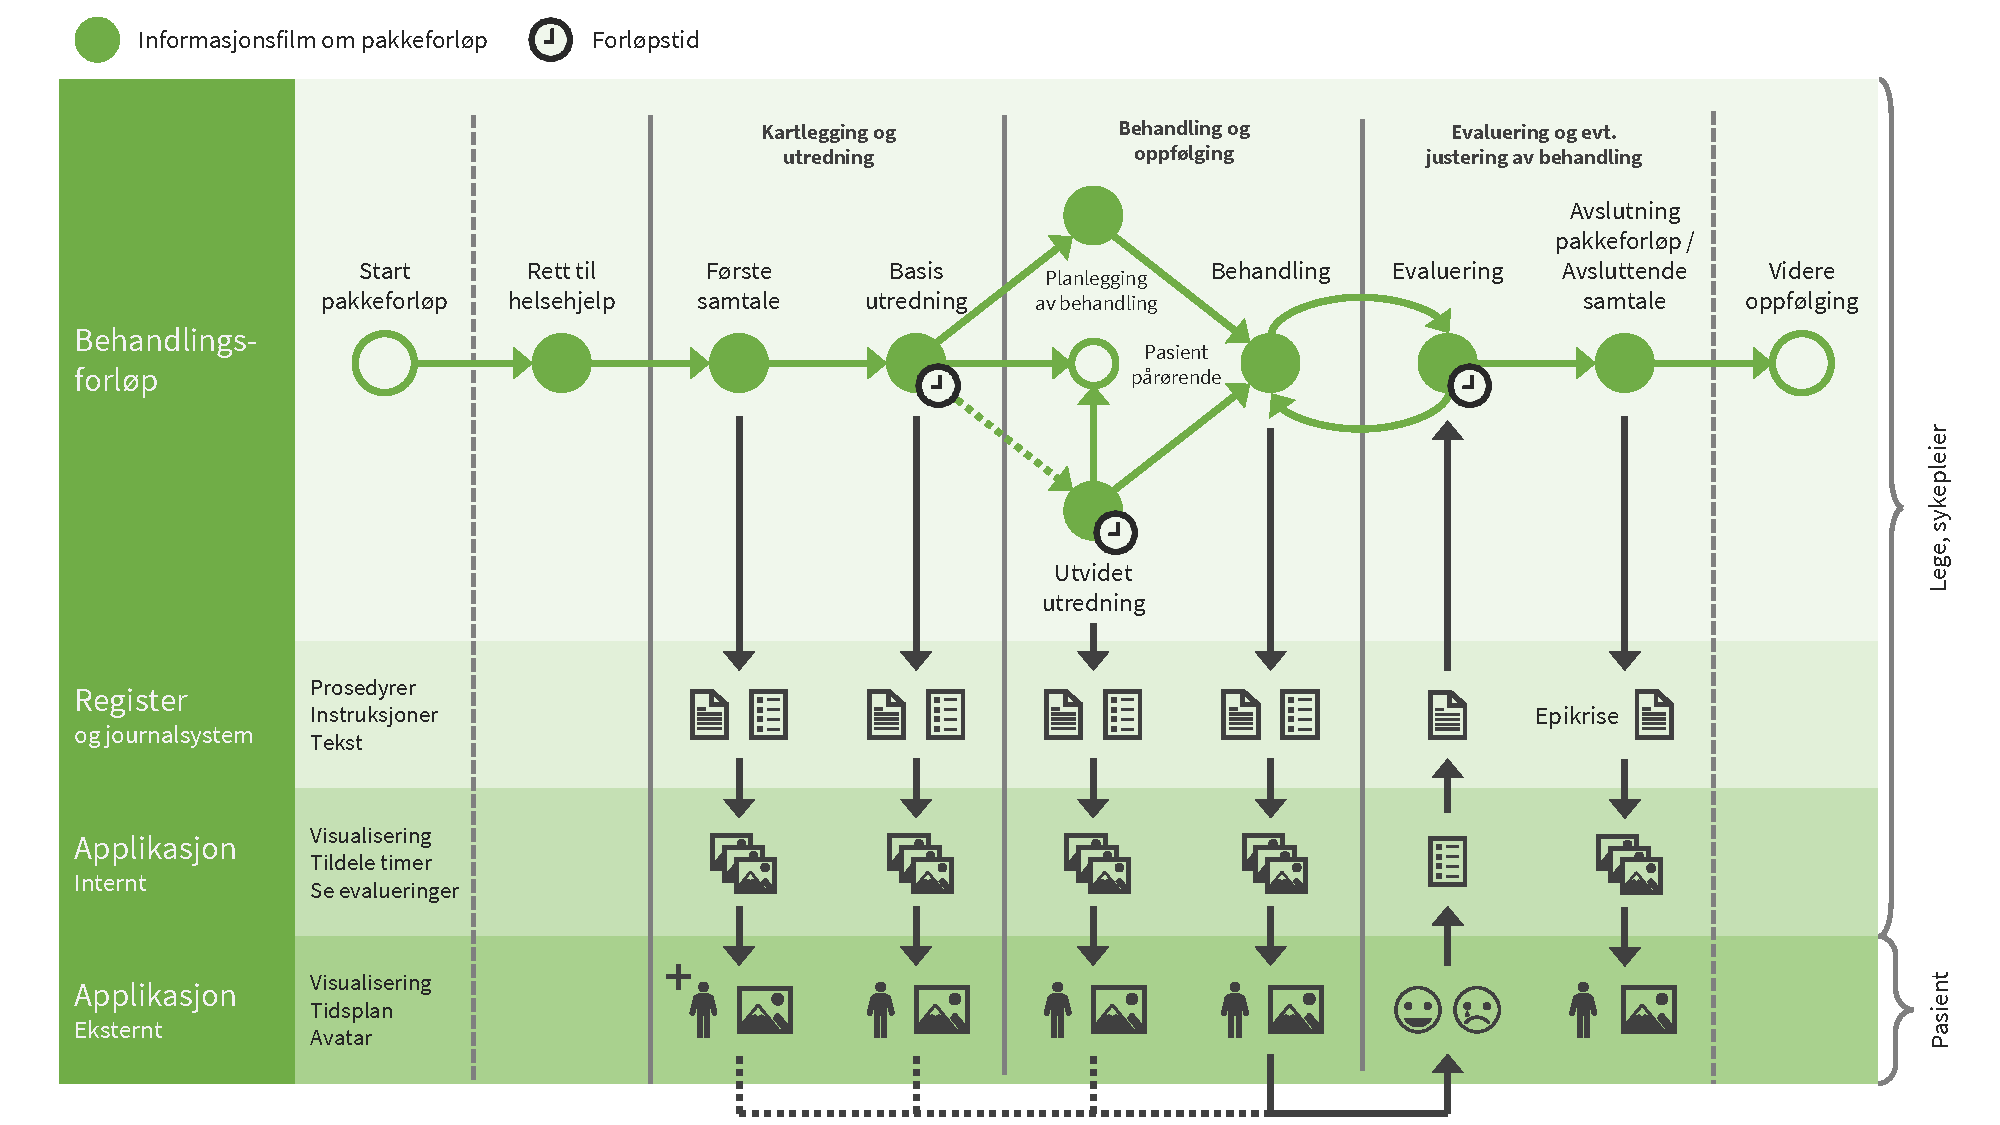
\includegraphics[width=1\textwidth]{application-model.pdf}
    \caption{Application model as illustrated through a guideline pathway}
    \label{fig:applicationmodel}
\end{figure}

The application is also to be integrated with existing information and journal systems. Details about these are not widely known and thus only speculations can be made. Information about procedures and appointments are fetched from these systems, updated as necessary. The graphical procedures are currently meant to be stored separately in the NoSQL database. Ratings can also be reflected in journals, supplying an extra dimension to each patient's journal. If this information can be stored in journals, there is a possibility that these journals can function as a storage for ratings and the likes. How the connections themselves are made is yet to be investigated.

\section{Anticipated challenges and feasibility}
\label{sec:anticipatedchallenges}

The development tools chosen for an application should support the functionality of the application. The following subsections illustrate a few scenarios which the chosen development tools should support.

\subsection{Personalised avatars}

The avatar generation system created for E-LAN (from \autoref{sec:relatedwork}) can be used together with the application. This enables the user to view their avatar in procedures like they were participating themselves. A challenge lies in associating an avatar to each user while making it easy to modify it when needed. The system is based on a graphical user interface and does not present an API; it is very much a black box where the result is a single layer of raster graphics.

\subsection{Realistic avatar projections}

The system outputs two-dimensional portrait images only, with the face and chest facing forward. The images are also limited to the top part of the body, leaving the lower body out. Concerns were raised about whether these images would look realistic in certain settings. For example, using a single 2D image, a person laying in the bed would look awkward unless viewed from above the bed. \Cref{tab:projecting-avatar} lists several approaches to this issue.

% Figure showing avatar

% Figure with 4 images showing the different projections?

\begin{table}
    \centering
    \begin{tabu}{L[0.75] l L[0.5] l L}
        \textbf{} & \textbf{Realism} & \textbf{Processing \newline power} & \textbf{Ease of use} & \textbf{Additional \newline requirements} \\ \hline
        \textbf{2D images} & Lowest & Lowest & Highest & None \\ \tabucline[hdottedline]{-}
        \textbf{2D image sets with various poses} & High & Low & High & Extra image sets \\ \tabucline[hdottedline]{-}
        \textbf{2D images rotated in 3D} & Low & High & Low & Software framework which supports 3D rotations \\ \tabucline[hdottedline]{-}
        \textbf{3D models} & Highest & Highest & Lowest & New 3D models; a 3D rendering engine; software framework which supports 3D rotations \\ \hline
    \end{tabu}
    \caption{Different ways to project an avatar on a screen}
    \label{tab:projecting-avatar}
\end{table}

It is shown that 2D images can be rotated in 3D pretty realistically. \textcite{rivers2010} carried out a project which showed that it is possible to view a figure from any angle when given three 2D projections of it. Though, an alternative is to simply use such avatars in 2D-space. The IACTA application shows that this can be used with similar effect as a 3D-application \autocite{stalberg2018}.

\subsection{Visual art and template designs}

This kind of application demands a lot of visual art, most notably in procedures but also in avatars if the avatar generation system is to be updated. The creation of visual art does not come for free; one would either need to purchase art bundles or hire a designer for this task.

\subsection{Connections between client and administrator applications}

When an administrator publishes and schedules a new procedure, it should quickly appear for the corresponding patient. This sets some requirements for the architecture. Once a new procedure is out, the patient's page should be updated to reflect any changes -- even if the web page is already open.

\subsection{Integrations towards current healthcare systems}

As mentioned in \autoref{sec:integration}, integrations toward healthcare systems remain. The challenge lies in the fact that journal systems are big. When tackling this risk, one should also consider the fact that journal systems may be updated.

\subsection{Security concerns}

Additional measures may be necessary in order to restrict unauthorized access to the application. This is a matter for both administrator and patient aspects as any unauthorized access to these would be catastrophic. If possible, users may be checked against national authorization systems such as BankID for verifying their identities -- even only for once.

\subsection{Service workers and offline content}

Offline content has always been a challenge for web applications, although the recent addition of \emph{service workers} make it easier. The technology is still new and experimental with varying (but improving) browser support, thus extensive testing may be needed to determine if the application can run completely offline.

\subsection{Scaling}

Depending on the network traffic, it may be necessary to design a scalable architecture. The scaling may be done through load balancers as previously suggested, or through scalable clusters in a container-orchestration system. More knowledge about the network traffic at the Children and Youth Clinic is needed.

\subsection{Costs}

An application of this size does not come without a significant price tag. Expenses include development team salaries, visual art, hosting and scaling. One needs to weight these expenses up with incomes (or projected incomes) in order to find out whether the application will be profitable. Investigating business models and budget variants which take incomes and expenses into consideration is suggested here.

% \section{Handoff}

% and source code for an incomplete software prototype using React and create-react-app.
